Figure \ref{fig:beat-frequency} illustrates the transmitted chirp and and the reflected echo
from one target. After converting the received echo to baseband signal,
the frequency of the resulting signal will be the difference between the currently transmitted signal and received echo.
This frequency is called the beat frequency $\gls{beatfreq}(t)$.

Given the signal is sampled $\gls{numsamples}$ times during a single chirp with a sampling frequency of \gls{samplerate},
the discrete Fourier transform will result in $\gls{numsamples}$ range bins,
hence the resolution of the Fourier transform is as given by equation \ref{eq:beat-frequency-resolution}.
\begin{equation}
    \label{eq:beat-frequency-resolution}
    \gls{beat-resolution} = \frac{\gls{samplerate}}{\gls{numsamples}}
\end{equation}

\begin{figure}
    \centering
    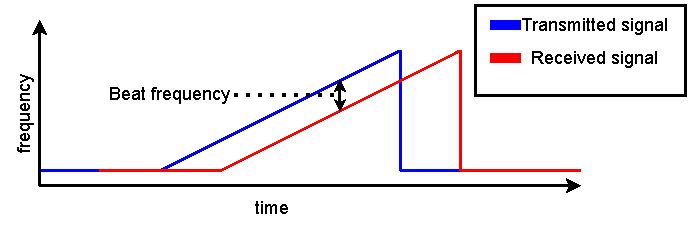
\includegraphics[width=0.8\textwidth]{fig/appendices/beat-frequency.pdf}
    \caption{Transmitted signal, reflected echo, and beat frequency.}
    \label{fig:beat-frequency}
\end{figure}

\section{Deriving the range equation}
Assuming the radar is of monostatic kind and not moving,
the beat frequency is produced solely by the delay caused by the round-trip-time from the radar to the target and back
and the Doppler-shift caused by the target.
Assuming the signal is propagating at the speed of light, the round-trip-time $\gls{roundtriptime}$ is given by equation \ref{eq:beat-frequency-rtt},
and the Doppler-shift $\gls{dopshift}$ by equation \ref{eq:beat-frequency-doppler},
where $\gls{range-l}$ is the range to the $l$:th target.
\begin{equation}
    \label{eq:beat-frequency-rtt}
    \gls{roundtriptime} = \frac{2\gls{range-l}}{\gls{lightspeed}}
\end{equation}

\begin{equation}
    \label{eq:beat-frequency-doppler}
    \gls{dopshift} = \frac{\gls{velocity}_{l}}{\gls{lightspeed}}\gls{txfreq}
\end{equation}

Because the slope $\gls{slope}$ of the signal is constant,
the beat frequency is linearly proportional to round-trip time.
The beat frequency of the reflection from the $l$:th target 
is given by equation \ref{eq:frequency-at-receiver}.
\begin{equation}
    \label{eq:frequency-at-receiver}
    \gls{beatfreq-l} = s \frac{2 \gls{range-l}}{\gls{lightspeed}} + \gls{dopshift-l}
\end{equation}

When the doppler shift of the $l$:th target is much lower than the beat frequency resolution, 
i.e. $\gls{dopshift-l} \ll \gls{beat-resolution} $, the equation \ref{eq:frequency-at-receiver} can be approximated
as given by equation \ref{eq:frequency-at-receiver-approx},
thus the range of the target on range $\gls{range-l}$ is given by equation \ref{eq:target-range-fft}.
\begin{equation}
    \label{eq:frequency-at-receiver-approx}
    \gls{beatfreq-l} \approx \frac{2 \gls{range-l} \gls{slope}}{\gls{lightspeed}}
\end{equation}
\begin{equation}
    \label{eq:target-range-fft}
    \gls{range-l} \approx \frac{\gls{beatfreq-l} \gls{lightspeed}}{2\gls{slope}}
\end{equation}

By combining the equations \ref{eq:beat-frequency-resolution} and \ref{eq:target-range-fft},
the range resolution of the fast-time Fourier transform is given by \ref{eq:range-resolution}.
\begin{equation}
    \label{eq:range-resolution}
    \gls{range-resolution} = \frac{\gls{beat-resolution} \gls{lightspeed}}{2\gls{slope}}
\end{equation}

Due to complex sampling, the maximum frequency observable by the receiver is
equal to the sampling frequency. Thus, the maximum beat frequency and thereby maximum range is dictated
by the sampling frequency \gls{samplerate}. The maximum range is given by equation \ref{eq:max-range}.
\begin{equation}
    \label{eq:max-range}
    \gls{maxrange} = \frac{\gls{samplerate} \gls{lightspeed}}{2\gls{slope}}
\end{equation}

\section{Velocity equation}
The change of the phase of a signal after it has been transmitted
is given by the wavelength and distance travelled (equation \ref{eq:phase-range-relation}).
Upon reflection, the signal experiences a phase change of $\pi$ radians and the frequency of the signal
changes due to Doppler shift.
\begin{equation}
    \label{eq:phase-range-relation}
    \gls{phase-change} (\gls{range}, \gls{txfreq}) = 2\pi \left( \frac{\gls{range}}{\gls{wavelen}} - \left\lfloor \frac{\gls{range}}{\gls{wavelen}} \right\rfloor \right)
    = 2\pi \left( \frac{\gls{txfreq}\gls{range}}{\gls{lightspeed}} - \left\lfloor \frac{\gls{txfreq}\gls{range}}{\gls{lightspeed}} \right\rfloor \right)
\end{equation}

Equation \ref{eq:phase-range-relation} is a surjection but not a bijection,
thus the range of the target cannot be determined from the range unless it is less than the wavelength
when the floor function term ($\lfloor \cdot \rfloor$) becomes zero and the function becomes a bijection.
The special case is shown by equation \ref{eq:phase-range-relation-special-case}.
\begin{equation}
    \label{eq:phase-range-relation-special-case}
    \forall \gls{range} \in [0, \gls{wavelen}] : \gls{phase-change} (\gls{range}, \gls{txfreq}) = 2\pi \frac{\gls{txfreq}\gls{range}}{\gls{lightspeed}} 
\end{equation}

When the signal reflects off a target, it experiences a phase change of $\pi$ radians.
The phase of the received reflection is thus given by equation \ref{eq:received-phase}

\begin{equation}
    \label{eq:received-phase}
    \gls{phase-rx}(\gls{range},\gls{txfreq}) = \gls{phase-tx}
    + \gls{phase-change} (\gls{range}, \gls{txfreq}) + \pi + \gls{phase-change}(\gls{range}, \gls{txfreq}+\frac{\gls{velocity}}{\gls{lightspeed}}\gls{txfreq})
\end{equation}

Because phase is linearly proportional to range,
as shown by equation \ref{eq:phase-range-relation-special-case},
the phase difference between the signals reflected from two targets moving at the same velocity
can be calculated as shown by equation \ref{eq:phase-diff-to-range-diff}.

\begin{equation}
    \label{eq:phase-diff-to-range-diff}
    \begin{aligned}
    \Delta \phi(\gls{range}_1, \gls{range}_2,\gls{txfreq}) &= \gls{phase-change}(\gls{range}_1, \gls{txfreq}) + \pi + \gls{phase-change}(\gls{range}_1, \gls{txfreq}+\frac{\gls{velocity}}{\gls{lightspeed}}\gls{txfreq}) \\
        &- \left( \gls{phase-change}(\gls{range}_2, \gls{txfreq}) + \pi + \gls{phase-change}(\gls{range}_2, \gls{txfreq}+\frac{\gls{velocity}}{\gls{lightspeed}}\gls{txfreq})  \right) \\
        &= \gls{phase-change}(\gls{range}_1, \gls{txfreq}) + \gls{phase-change}(\gls{range}_1, \gls{txfreq}+\frac{\gls{velocity}}{\gls{lightspeed}}\gls{txfreq}) \\
        &- \gls{phase-change}(\gls{range}_2, \gls{txfreq}) - \gls{phase-change}(\gls{range}_2, \gls{txfreq}+\frac{\gls{velocity}}{\gls{lightspeed}}\gls{txfreq}) 
    \end{aligned}
\end{equation}

Again assuming $\gls{range}_1 - \gls{range}_2 < \gls{wavelen}$, the equation \ref{eq:phase-diff-to-range-diff} can be evaluated as
given by equation \ref{eq:phase-diff-to-range-diff-expanded}.

\begin{equation}
    \label{eq:phase-diff-to-range-diff-expanded}
    \begin{aligned}
        \forall \gls{range}_1 &- \gls{range}_2 \in [0, \gls{wavelen}] : \gls{phase-change}(\gls{range}_1, \gls{range}_2, \gls{txfreq}) \\
        &= 2\pi \gls{txfreq} \gls{range}_1 \left( \frac{1+\frac{\gls{velocity}}{\gls{lightspeed}} }{\gls{lightspeed}} \right)
        - 2\pi \gls{txfreq} \gls{range}_2 \left( \frac{1+\frac{\gls{velocity}}{\gls{lightspeed}} }{\gls{lightspeed}} \right) \\
        &= 2\pi \gls{txfreq} (\gls{range}_1-\gls{range}_2) \left( \frac{1+\frac{\gls{velocity}}{\gls{lightspeed}} }{\gls{lightspeed}} \right)
    \end{aligned}
\end{equation}

The frequency of a sinusoidal wave can be expressed as $\gls{txfreq} = \gls{phasevelocity} \div (2\pi)$,
where \gls{phasevelocity} is the phase velocity of the wave.
Given the phase difference of a single-tone signal sampled 
at a time interval of \gls{chirptime} is $\gls{phase-change}_{\gls{chirptime}}$,
the corresponding frequency can be calculated using equation \ref{eq:phase-diff-to-freq}.
\begin{equation}
    \label{eq:phase-diff-to-freq}
    \gls{phase-change}_{\gls{chirptime}} = 2 \pi \gls{txfreq} \gls{chirptime}
    \Leftrightarrow
    \gls{txfreq} = \frac{ \gls{phase-change}_{\gls{chirptime}} }{ 2\pi \gls{chirptime} }
\end{equation}

From the properties of discrete Fourier transform,
it is known that the frequency resolution for the transform is $\gls{freq-resolution} = 1 \div \gls{chirptime}$.
Because the target can have either a positive or negative velocity,
both positive and negative frequencies may be induced by the change in range.
Hence, the domain of interest for the slow-time Fourier transform is
$\gls{txfreq} \in [-\frac{1}{2\gls{chirptime}}, \frac{1}{2\gls{chirptime}}]$.
The corresponding set of phase shifts is $\gls{phase} \in [- \pi, \pi]$
and the phase resolution of the transform is $\gls{phase-change} = \frac{2\pi}{\gls{numchirps}}$.

Given the signal is sampled $\gls{numchirps}$ times at the rate of $\gls{chirptime}$,
the frequency resolution (\gls{freq-resolution}) for a discrete Fourier transform of the signal is $\gls{numchirps} \div \gls{chirptime}$.
Thus, the velocity required for a Doppler-shift to induce an error of one bin (\gls{v-err})
is given by equation \ref{eq:doppler-error-velocity}.
Given $\gls{numchirps} = 64$, $\gls{txfreq} = 60~\mathrm{GHz}$ and $\gls{chirptime} = 260~\mathrm{\mu s}$
(realistic values for an \gls{fmcw} radar), $\gls{v-err} \approx 1230~\frac{\mathrm{m}}{\mathrm{s}}$.
\begin{equation}
    \label{eq:doppler-error-velocity}
    \frac{\gls{v-err}}{\gls{lightspeed}}\gls{txfreq} = \frac{\gls{numchirps}}{\gls{chirptime}}
    \Leftrightarrow 
    \gls{v-err} = \frac{\gls{lightspeed}\gls{numchirps}}{\gls{txfreq} \gls{chirptime}}
\end{equation}

Given $v \ll v_\mathrm{err}$, the equation \ref{eq:phase-diff-to-range-diff-expanded}
can be approximated as given by equation \ref{eq:phase-diff-to-range-diff-expanded-approx}.
\begin{equation}
    \label{eq:phase-diff-to-range-diff-expanded-approx}
    \begin{aligned}
        \forall \gls{range}_1 &- \gls{range}_2 \in [0, \gls{wavelen}] : \Delta \phi(\gls{range}_1, \gls{range}_2 ,\gls{txfreq}) \\
        &= \frac {2\pi \gls{txfreq} (\gls{range}_1-\gls{range}_2)}{\gls{lightspeed}}
    \end{aligned}
\end{equation}

Substituting $\gls{phase-change}$ in equation \ref{eq:phase-diff-to-range-diff-expanded-approx}
with the frequency resolution and denoting $\gls{range}_1 - \gls{range}_2 = 2 \gls{range-resolution}$ 
(change in target range causes twice the change in propagation distance),
the equation can be solved for $\gls{range-resolution}$ to acquire the range resolution
for the slow-time Fourier transform. Dividing the value with the sampling interval $\gls{chirptime}$,
the minimum and maximum velocity and the velocity resolution can be calculated as given by equations
\ref{eq:slow-time-velocity-resolution} and \ref{eq:slow-time-velocity-max}.
\begin{equation}
    \label{eq:slow-time-velocity-resolution}
    \gls{velocity-resolution} = \frac{\gls{phase-change} \gls{lightspeed}}{4 \pi \gls{txfreq} \gls{chirptime}} 
    = \frac{2 \pi \gls{lightspeed}}{4 \gls{numchirps} \pi \gls{txfreq} \gls{chirptime}} 
    = \frac{\gls{lightspeed}}{2 \gls{numchirps} \gls{txfreq} \gls{chirptime}}
\end{equation}
\begin{equation}
    \label{eq:slow-time-velocity-max}
    \begin{cases}
        \gls{maxvelocity} = \frac{\gls{phase} \gls{lightspeed}}{4 \pi \gls{txfreq} \gls{chirptime}} = \frac{\gls{lightspeed}}{4 \gls{txfreq} \gls{chirptime}}\\
        \gls{minvelocity} = \frac{- \gls{phase} \gls{lightspeed}}{4 \pi \gls{txfreq} \gls{chirptime}} = \frac{-\gls{lightspeed}}{4 \gls{txfreq} \gls{chirptime}}
    \end{cases}
\end{equation}
